\section{Overview}
\label{sec:overview}

In this section, we illustrate our technique on the verification of 
correctness, in the sense of linearizability, of
a concurrent set data structure based on skiplists, namely the
Lock-Free Concurrent Skiplist from~\cite[Section 14.4]{ArtOfMpP}.
\begin{wrapfigure}{r}{0.5\textwidth} 
\vspace{-20pt}
  \begin{center}
 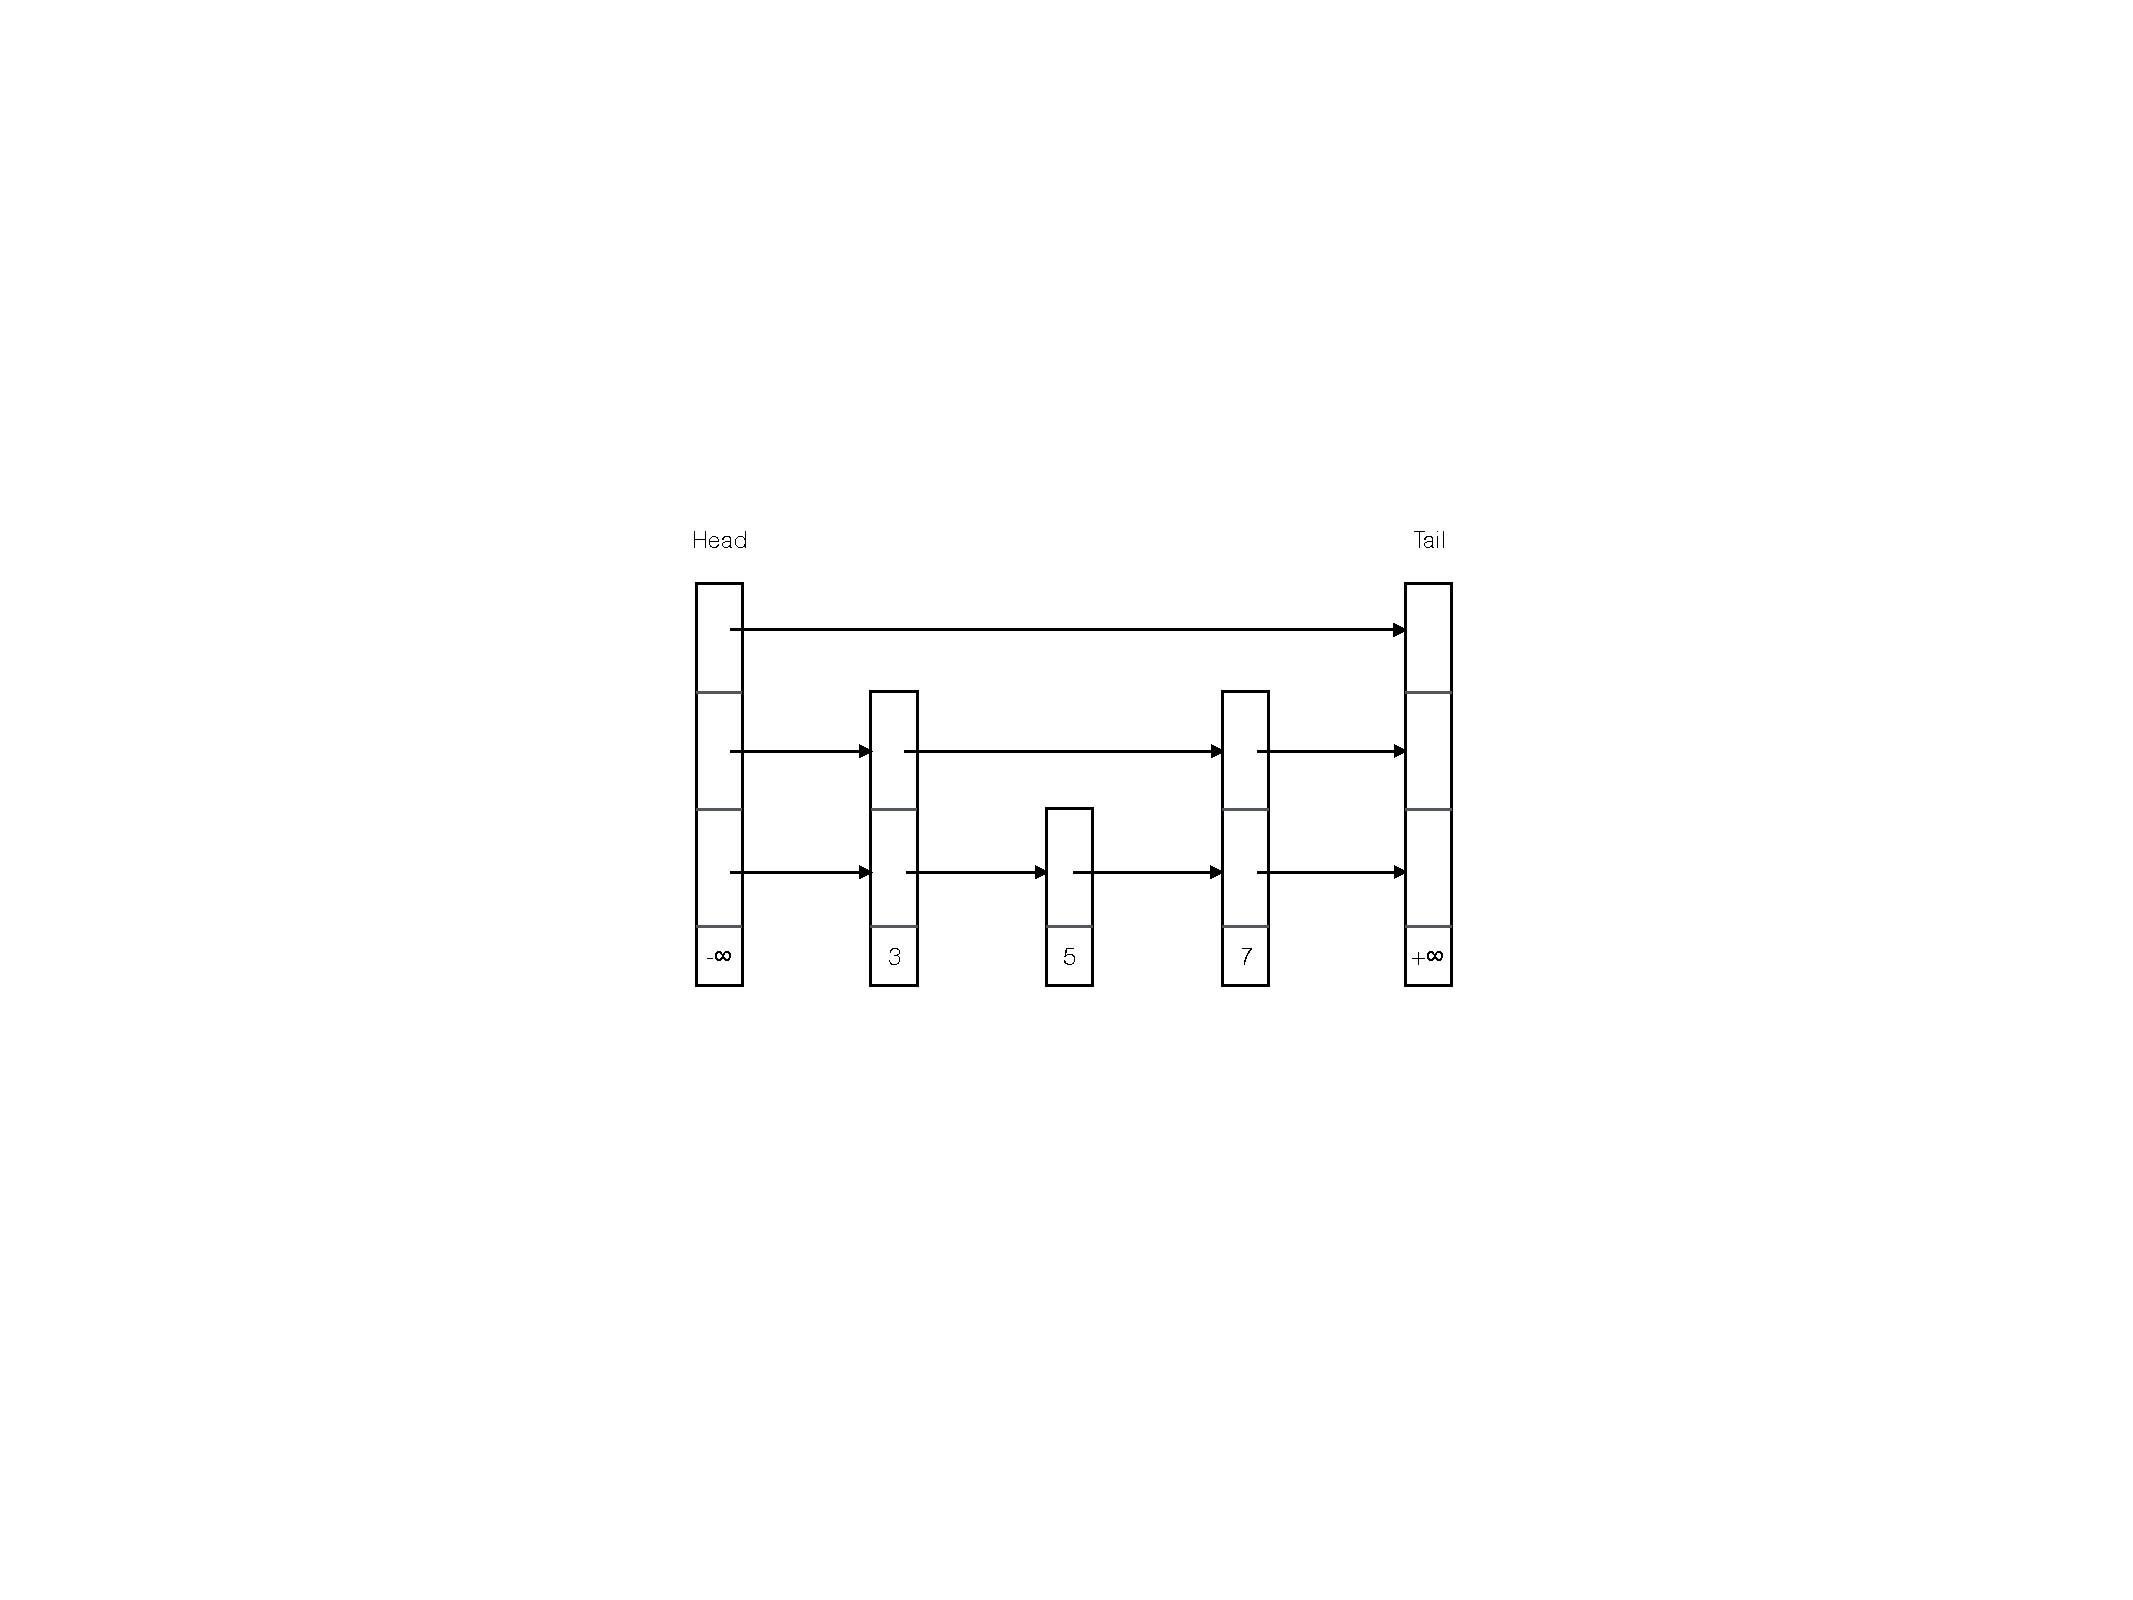
\includegraphics[width=0.5\textwidth, trim={11cm 10cm 10cm 9cm}, clip]{normalskipshape.pdf}  
    \caption{An example of skiplist}
    \label{normalskiplist}
  \end{center}
  \vspace{-35pt}
  \vspace{1pt}
\end{wrapfigure}
%\bjcom{Quy: I assume you will take care of this section}
Skiplists provide expected logarithmic time search while avoiding some of the complications of tree structures.
Informally, a skiplist consists of a collection of sorted linked lists, each of which is located at a {\em level}, ranging from $1$ up to a maximum value. Each skiplist node has a key value and participates in the lists at levels $1$ up to its {\em height}.
The skiplist has sentinel head and tail nodes with maximum heights and key values $-\infty$ and $+\infty$, respectively.
%Figure~\ref{sl} shows a skiplist with maximum height of 3.
The lowest-level list (at level $1$) constitutes an ordered list of all nodes
in the skiplist. Higher-level lists are increasingly sparse sublists of the
lowest-level list, and serve as shortcuts into lower-level lists. Figure~\ref{normalskiplist} shows an example of a skiplist of height 3. It has head and tail nodes of height $3$, two nodes of height $2$, and one node of height $1$.

The algorithm has three main methods, namely $\tt add$, $\tt contains$ and $\tt remove$. The method $\tt add(x)$ adds $\tt x$ to the set and returns true iff $\tt x$ was not already in the set; $\tt remove(x)$ removes $\tt x$ from the set and returns true iff ${\tt x}$ was in the set; and $\tt contains(x)$
returns true iff $\tt x$ is in the set.
All methods rely on a method $\tt find$ to search for a given key. 
In this section, we shortly describe the $\tt find$ and $\tt add$ methods.
Figure~\ref{sl-code:fig} shows code for these two methods.
\vspace*{-0.6cm}
%\bjcom{Start with the most important property of the method. What does it do?}
\input slcode


%\bjcom{Say how the list looks, and the role of marked nodes}

\vspace*{-0.6cm}

In the algorithm, each heap node has a $\tt key$ field, a $\tt height$, an array of $\tt next$ pointers indexed from
$1$ up to its $\tt height$, and an array of $\tt marked$ fields which are true if the node has been logically removed at the corresponding level. Removal of a node (at a certain level $\klevel$) occurs in two steps: first the node is logically removed by setting its $\tt marked$ flag at level $\klevel$ to $\tt true$, thereafter the node is physically removed by unlinking it from the level-$\klevel$ list. The algorithm must be able to update the $\tt next[k]$ pointer and $\tt marked[k]$ field together as one atomic operation; this is standardly implemented by encoding them in a single word. The head and tail nodes of the skiplist are pointed to by global pointer variables $\tt H$ and $\tt T$, respectively. The $\tt find$ method traverses the list at decreasing levels using two local variables $\tt pred$ and $\tt curr$, starting at the head and at 
the maximum level (lines 5-6). At each level $\tt k$ it sets $\tt curr$ to $\tt pred.next[k]$ (line 7). During the traversal, the pointer variable $\tt succ$ and boolean variable $\tt marked$ are atomically assigned the values of $\tt curr.next[k]$ and $\tt curr.marked[k]$, respectively (line 9, 14). After that, the method repeatedly removes marked nodes at the current level (lines 10 to 14). This is done by using a $\tt CompareAndSwap$ $\tt (CAS)$ command (line 11), which tests whether $\tt pred.next[k]$ and $\tt pred.marked[k]$ are equal to $\tt curr$ and $\tt false$ respectively. If this test succeeds, it replaces them with $\tt succ$ and $\tt false$ and returns $\tt true$; otherwise, the $\tt CAS$ returns $\tt false$. During the traversal at level $\tt k$, $\tt pred$ and $\tt curr$ are advanced until $\tt pred$ points to a node with the largest key at level $\tt k$ which is smaller than $\tt x$ (lines 15-18). Therafter, the resulting values of $\tt pred$ and $\tt curr$ are recorded into $\tt preds[k]$ and $\tt succs[k]$ (lines 19, 20), whereafter traversal continues one level below until it reaches the bottom level. Finally, the
method returns $\tt true$ if the $\tt key$ value of $\tt curr$ is equal to $\tt x$; otherwise, it returns $\tt false$ meaning that a node with key $\tt x$ is not found.


%% Once an unmarked $\tt curr$ is found (line 20), it is tested to see if its key is less than the target key. If so, $\tt pred$ is advanced to $\tt curr$. Otherwise, $\tt curr$'s key is greater than or equal to $\tt x$, so the current value
%% of $\tt pred$ is the target node's immediate predecessor. The method breaks out of the current level search loop, saving the current values of $\tt pred$ and $\tt curr$. It proceedsd int by this way until reaching the bottom level.

The $\tt add$ method uses $\tt find$ to check whether a node with key $\tt x$ is already in the list. If so it returns $\tt false$; otherwise, a new node is created with randomly chosen height $\tt h$ (line 7), and with $\tt next$ pointers at levels from $1$ to $\tt h$  initialised to corresponding elements of $\tt succ$ (line 8 to 9). Thereafter, the new node is added into the list by linking it into the bottom-level list between the $\tt preds[1]$ and $\tt succs[1]$ pointers returned by $\tt find$. This is achieved by using a $\tt CAS$ to make $\tt preds[1].next[1]$ point to the new node (line 13). If the $\tt CAS$ fails, the $\tt add$ method will restart from the beginning (line 3) by calling $\tt find$ again, etc. Otherwise, $\tt add$ proceeds with linking the new node into the list at increasingly higher levels (lines 16 to 22). For each higher level $\klevel$, it makes $\tt preds[k].next[k]$ point to the new node if it is still valid (line 20); otherwise
$\tt find$ is called again to recompute $\tt preds[k]$ and $\tt succs[k]$ on the remaining unlinked levels (line 22). Once all levels are linked, the method returns $\tt true$.

 
%The $\tt remove$ method also use $\tt find$ to determine whether an unmarked node with a matching key $\tt k$ is in the bottom-level list. If no node is found in the bottom-level list, or the node with a matching key is marked, the method returns false. If an unmarked node is found, then the method logically removes the associated key from the list, and prepares it for physical removal. First, starting from the topLevel, all links up to and not including the bottom-level link are marked . If the link is found to be marked the method moves on to the next-level link. Otherwise, the marking attempt must be repeated. Once all levels but the bottom one have been marked, the method marks the bottom level€™s next reference. Before returning true, the $\tt find$ method is called again. This call physically removes all links to the node it is searching for if that node is already logically removed.

%For each level, it attempts to set the predecessor, if it refers to the valid successor, to the new node . If successful, it moves on to the next level. If unsuccessful, the $\tt find$ method is called again to find a new valid position. 

%We use $\tt compareAndSet$ to set the reference while validating that these nodes still refer one to the other and have not been removed from the list. If the $\tt compareAndSet$ fails, the call restarts. 
%Figure~\ref{ts-stack:fig} shows a simplified version of the Timestamped Stack (TS stack), where we have omitted the check for emptiness in the ${\tt pop}$ method, and the optimization using ${\tt push}$-${\tt pop}$ elimination. These features are included in the full version of the algorithm, described in Appendix XXX, that we have verified automatically.
%
%The algorithm uses an array of singly-linked lists (SLLs), one for each thread, accessed via the thread-indexed array ${\tt pools[maxThreads]}$ of pointers to the first cell of each list. The ${\tt init}$ method initializes each of these pointers to $\nullconst$. Each list cell contains a data value, a timestamp value, a ${\tt next}$ pointer, and a boolean flag ${\tt mark}$ which indicates whether the node is logically removed from the stack. Each thread pushes elements to ``its own'' list, and can pop elements from any list.
%
%A ${\tt push}$ method for inserting a data element ${\tt d}$ works as follows: first, a new cell with element ${\tt d}$ and minimal timestamp ${\tt -1}$ is inserted at the beginning of the list indexed by the calling thread (line 1-3). After that, a new timestamp is created and assigned (via the variable ${\tt t}$) to the ${\tt ts}$ field of the inserted cell (line 4-5).
%%\bjcom{Quesion to Quy: What happens when pop methods sees uninitialized timestamps?} \quycom{uninitialized time is -1, its smaller than any other time.}
%Finally, the method unlinks (i.e., physically removes) all cells that are reachable (through a sequence of $\tt next$ pointers) from the inserted cell and whose ${\tt mark}$ field is ${\tt true}$; these cells are already logically removed. This is done by redirecting the $\tt next$ pointer of the inserted cell to the first cell with a $\false$ $\tt mark$ field, which is
%reachable from the inserted cell.
%
%A ${\tt pop}$ method first traverses all lists, finding in each list
%the first cell whose ${\tt mark}$ field is ${\tt false}$(line 8), and letting the variable ${\tt youngest}$ point to the most recent such cell
%(i.e., with the largest timestamp) (line 1-11).
%A compare-and-swap (CAS) is used
%to set the ${\tt mark}$ field of this youngest cell to $\true$,
%thereby logically removing it.
%This procedure will restart if the CAS fails. After the youngest cell has been removed, the method will unlink all cells, whose ${\tt mark}$ field is ${\tt true}$,
%that appear before (line 17-19) or after (line 20-23) the removed cell.
%Finally, the method returns the ${\tt data}$ value of the removed cell.
%%\todo[inline]{Comments by Bengt: How can you return empty? Also, I think you
%% need to explain the extra removal of marked cells better} \quycom{this code is a simplified version without emptiness checking. If we add emptiness part, the code will be longer and more complicated}

To prepare for verification, we add a specification which expresses that
the skiplist algorithm of Figure~\ref{sl-code:fig} is a
linearizable implementation of a set data structure, using
the technique of
{\em observers}~\cite{AHHR:integrated,BEEH:icalp15,HSV:concur13,Quy:sas16}.
For our skiplist algorithm, the user first instruments statements in each
method that correspond to linearization points (LPs), so that their execution
announces the corresponding atomic set operation.
In Figure~\ref{sl-code:fig}, the LP of a successful ${\tt add}$ operation is at line 15 of the $\tt add$ method (denoted by a blue dot) when the $\tt CAS$ succeeds, whereas the LP of an unsuccessful $\tt add$ operation is at line 4 of the $\tt add$
method (denoted by a red dot).
We must now verify that in any concurrent
execution of a collection of method calls, the sequence of announced
operations satisfies the semantics of the set data structure.
This check is performed by an {\em observer}, which
monitors the sequence of announced operations. The observer for the set
data structure utilizes a register, which is initialized with
a single, arbitrary $\tt key$ value.
It checks that operations on this particular value follow set semantics,
i.e., that successful $\tt add$ and $\tt remove$ operations on an element alternate and that
$\tt contains$ are consistent with them.
We form %% as in the automata-theoretic approach~\cite{VW:modelchecking}
%% (adapted in~\cite{AHHR:integrated}),
the cross-product of the program  and the observer, synchronizing on
operation announcements. This reduces the
problem of checking linearizability to the problem of checking that
in this cross-product, regardless of the initial observer register value, the observer cannot reach a state where
the semantics of the set data structure has been violated.

%% In conclusion, verifying linearizability for skiplist-based set implementations
%% requires the user to associate linearization points with statements in the
%% methods of the implementation: the remaining steps are then automated.
%% We remark that this user annotation is not necessary when verifying
%% linearizability of stack and queue implementation. 
%% This is achieved by exploiting recent results saying that
%% linearizability for stacks and queues can be precisely specified by
%% observers that process the sequence of call and return actions of
%% methods,  instead of the user-supplied LPs~\cite{BEEH:icalp15,HSV:concur13}.
%% We use this technique for stacks and queues in Section XXX.

%% typically by affixing
%%   linearization points to particular statements, or in more complex cases by
%%   light-weight instrumentation using the approach of
%%   controllers~\cite{Quy:sas16}.

%% For many data structure implementations, LPs can be statically
%% affixed to particular statements in method implementations,
%% implying that correctness can be formulated as constraints on the ordering of the
%% occurrences of LPs in any program execution.
%% a concept of data-independence, these constraints can be formulated as
%% a number of samll observers, which are automata that recognize violations
%% of these ordering requirements~\cite{AHHR:integrated}.
%% does not LPs cannot be affixed to particular statements. For instance,  two overlapping
%% push operations may have to be linearized in different orders depending
%% on how their corresponding later pop operations are ordered in time.
%% not be determined during their invocation, but only later
%% when the ordering between the two corresponding pop operations is determined.
%% Instead, we use a recent technique of~\cite{BEEH:icalp15,HSV:concur13}, who show
%% that for stacks and queues,
%% linearizability can be precisely specified by a small number of
%% constraints on the ordering of call and return actions of the methods,
%% without any reference to LPs.


%% \begin{wrapfigure}{r}{.55\textwidth}
%% {\em Observers} are
%% finite automata extended with a finite set of {\em registers}
%% that assume values in $\intgrs$, which are 
%% nondeterministically initialized with arbitrary values, which never change
%% during a run of the observer. 
%% The observer accepts a trace if, for {\em some} initial values of the
%% registers, the trace can  be processed in such a way that
%% an accepting state is reached.
%% In other words, the observer is defined in such a way that it accepts precisely those
%% traces that do {\em not} belong to the behavior
%% of the data structure.
%% %% Observers can be used to give {\it exact} specifications of
%% %% the behaviors of data structures such as sets, queues, and stacks.
%% %
%% %
%% Fig.~\ref{set:observer:fig}
%% depicts an observer that accepts the
%% sequences of operations that do {\em not} conform to the semantics of a set
%% data structure.


%% In more complex cases, we use
%%   light-weight instrumentation using the approach of
%%   controllers~\cite{Quy:sas16}, which puts a small burden on
%%   the verifier. This is used in Section XXX for the verification of some
%%   implementations of sets based on singly-linked lists.

%% For concurrent data structures, one must be careful to 
%% expressed it exactly in terms of allowed sequences of calls
%% and returns of different methods. For completeness, we here
%% present how this can be done for a stack implementation, as shown
%% in~\cite{BEEH:icalp15}.
%% show how this can be done using observers, introduced in~\cite{AHHR:integrated}. 

%% Let $\calltwo{\tt push}{\tt d}$ and $\returntwo{\tt push}{\tt d}$ denote the
%% action of calling or returning from a ${\tt push}$ method with data parameter ${\tt d}$.
%% Let $\calltwo{\tt pop}{\tt d}$ and $\returntwo{\tt pop}{\tt d}$ denote the
%% action of calling or returning from a ${\tt pop}$ method which returns
%% the value ${\tt d}$.
%% %% Let a call action on an operation $\mname(\data)$ be denoted
%% %% $\calltwo{\mname}{\data}$ and a return action be denoted
%% %% $\returntwo{\mname}{\data}$.
%% Constraints on the ordering of such actions can be
%% checked by an {\em observer}.
%% %
%% Observers are
%% finite automata extended with a finite set of {\em registers} whose values range
%% over the domain of data values.
%% %
%% At initialization,
%% the registers are nondeterministically
%% assigned arbitrary distinct data values, which never change
%% during a run of the observer. 
%% %
%% %% Formally, an observer $\observer$ is a tuple
%% %% $\otuple$ where $\ostateset$ is a finite set 
%% %% of {\it observer states} including the 
%% %% {\it initial state} $\oinitstate$ and
%% %% the {\it accepting state} $\oaccstate$, 
%% %% a finite set $\ovarset$  
%% %% of {\it registers}, and $\otransitionset$ is a finite
%% %% set of {\it transitions}.
%% %% %
%% %% %
%% %% Transitions are of the form 
%% %% $\tuple{\ostate_1,\mname(\inxvar,\outxvar),\ostate_2}$ where 
%% %% $\inxvar$ and $\outxvar$ are either registers or constants, i.e.,
%% Transitions are labeled by actions parameterized by registers.
%% %% is the value of a register parameterized on registers.%
%% The observer processes a sequence of actions, one action at a time.
%% If there is a transition, whose label, after replacing registers by their
%% values, matches the action, such a transition is performed; otherwise
%% the observer remains in its current state.
%% %% %
%% %% If there is no
%% %% such transition, 
%% %
%% The observer accepts a sequence of actions
%% if, for some initial assignment of data values to its registers, the sequence
%% can be processed in such a way that an accepting state is reached.
%% The observer for a particular constraint is defined in such a way that it
%% accepts precisely those sequences  that do {\em not} satisfy the constraint.


%% \begin{figure}
%% \center 

%% \begin{tikzpicture}[]

%% \node(s0)[draw,line width=0.5pt,circle,text=black]
%% {$s_0$};

%% \node(s2)[draw,line width=0.5pt,circle,text=black,anchor=center]
%% at ($(s0.center)+(40pt,50pt)$) {$s_2$};



%% \node(s1)[draw,line width=0.5pt,circle,text=black,anchor=center]
%% at ($(s0.center)+(80pt,0pt)$) {$s_1$};

%% \node(init)[line width=0.5pt,circle,text=black,anchor=center]
%% at ($(s0.center)+(-30pt,0pt)$) {};
%% \draw[->,>=stealth,line width=0.5pt] (init) to 
%% node[left=5pt,pos=0.5] {} 
%% (s0);

%% \node[draw,line width=0.5pt,circle,text=black,anchor=center,minimum size=5mm]
%% at ($(s0.center)+(80pt,0pt)$) {};


%% \draw[->,>=stealth,line width=0.5pt,] (s0) to 
%% node[above=-1pt,pos=0.5] {\footnotesize${\tt ret \; pop}(x)$} 
%% (s1);

%% \draw[->,>=stealth,line width=0.5pt] (s0) to 
%% node[left=5pt,pos=0.5] {\footnotesize${\tt call \; push}(x)$} 
%% (s2);

%% \draw[->,>=stealth,line width=0.5pt, in=-50,out=-130,loop] (s0) to 
%% node[above=-15pt,pos=0.5] {\footnotesize${\tt call \; pop}(x)$} 
%% (s0);

%% %% \draw[->,>=stealth,line width=0.5pt, in=50,out=-30,loop] (s2) to 
%% %% node[right=2pt,pos=0.5] {\footnotesize${\tt act(x)}$} 
%% %% (s2);


%% %\node[]
%% %at ($(s2.center)+(60pt,20pt)$) {\footnotesize${\tt call \; push}(x)+$};
%% %\node[] at ($(s2.center)+(60pt,10pt)$) {\footnotesize${\tt ret \; push}(x)+$};
%% %\node[] at ($(s2.center)+(60pt,0pt)$) {\footnotesize${\tt call \; pop}(x)+$};
%% %\node[] at ($(s2.center)+(60pt,-10pt)$) {\footnotesize${\tt ret \; pop}(x)$};

%% \end{tikzpicture}
%% \caption{An observer recognizing sequences in which ${\tt pop}$ for some data value returns although no
%%   corresponding ${\tt push}$ has been previously called. The observer has one register $\tt x$.}
%% \label{fig:nonpopobserver:fig}
%% \end{figure}

%% %\todo[inline]{Quy: make a picture of this observer, and describe intuitively
%% %  how it works}


%% %\todo[inline]{The observer of Fig. 2 is not correct: You must also include
%% %  call push(x) which goes to a sink state. Moreover, you must explain that you
%% %  assume differentiated traces, Plese go over the observer again. Also mark
%% %  the initial location}

%% As an example, Figure~\ref{fig:nonpopobserver:fig} shows an observer for
%% Constraint 1, which checks
%% that a ${\tt pop}$ method must not return before any ${\tt push}$ method
%% with the same data value has been called.
%% %% The exact form of observers for these constraints represent them in
%% %% terms of ordering of call an return actions.
%% Observers for Constraints 2 and 3 are similar to that for Constraint 1.
%% The observer for Constraint 4 is more complex,
%% and shown in Figure~\ref{fig:lifostack:fig}.
%% It has two registers $\tt x_1$ and $\tt x_2$. Let $\tt d_1$ and $\tt d_2$
%% denote their initial values.
%% In a sequence of actions that leads to the accepting state $s_6$, a
%% ${\tt push(d_1)}$ must be linearized before a ${\tt push(d_2)}$, since
%% ${\tt push(d_1)}$ returns before ${\tt push(d_2)}$ is called; however
%% a ${\tt pop(d_1)}$ returns in a situation where the number of returned
%% ${\tt push(d_2)}$ methods exceeds the number of called
%% ${\tt pop(d_2)}$ methods, thereby violating LIFO ordering.
%% %% ${\tt pop(d_2)}$ which leaves some data value $\tt d_2$ on top of
%% %% $\tt d_1$ in the stack, also violating LIFO ordering.
%% %% In the observer, the action which leads to an accepting state $\tt ret \; pop(x_1)$ happens after sequences of actions namely $\tt call \; push(x_2)$, $\tt ret \; push(x_2)$, $\tt call \; pop(x_2)$ in which the pair $\tt ret \; push(x_2) / call \; pop(x_2)$ is always after $\tt ret \; push(x_2)$ . The $\tt call \; push(x_1)/ret \;push(x_1)$ happens before all the sequences. Intuitively, the observer specifies that a data cannot be popped from the stack if there is always at least an different data above it in the Stack (regardless of how linearize the execution). 
%% %\todo[inline]{The explanation of Figure 3 to be improved}
%% \begin{figure}
%% \center 

%% \begin{tikzpicture}[]

%% \node(s0)[draw,line width=0.5pt,circle,text=black]
%% {$s_0$};


%% \node(s1)[draw,line width=0.5pt,circle,text=black,anchor=center]
%% at ($(s0.center)+(60pt,0pt)$) {$s_1$};

%% \node(s2)[draw,line width=0.5pt,circle,text=black,anchor=center]
%% at ($(s0.center)+(120pt,0pt)$) {$s_2$};

%% \node(s3)[draw,line width=0.5pt,circle,text=black,anchor=center]
%% at ($(s0.center)+(180pt,0pt)$) {$s_3$};

%% \node(s4)[draw,line width=0.5pt,circle,text=black,anchor=center]
%% at ($(s0.center)+(240pt,0pt)$) {$s_4$};

%% \node(s6)[draw,line width=0.5pt,circle,text=black,anchor=center]
%% at ($(s0.center)+(300pt,0pt)$) {$s_6$};

%% \node(s5)[draw,line width=0.5pt,circle,text=black,anchor=center]
%% at ($(s0.center)+(240pt,-100pt)$) {$s_5$};

%% \node[draw,line width=0.5pt,circle,text=black,anchor=center,minimum size=5mm]
%% at ($(s0.center)+(300pt,0pt)$) {};


%% \draw[->,>=stealth,line width=0.5pt,] (s0) to 
%% node[above=-1pt,pos=0.5] {\tiny${\tt call \; push}(x_1)$} 
%% (s1);
%% \draw[->,>=stealth,line width=0.5pt,] (s1) to 
%% node[above=-1pt,pos=0.5] {\tiny${\tt ret \; push}(x_1)$} 
%% (s2);

%% \draw[->,>=stealth,line width=0.5pt,] (s2) to 
%% node[above=-1pt,pos=0.5] {\tiny${\tt ret \; push}(x_2)$} 
%% (s3);

%% \draw[->,>=stealth,line width=0.5pt,] (s3) to 
%% node[above=-1pt,pos=0.5] {\tiny${\tt call \; pop}(x_1)$} 
%% (s4);

%% \draw[->,>=stealth,line width=0.5pt,] (s4) to 
%% node[above=-1pt,pos=0.5] {\tiny${\tt ret \; pop}(x_1)$} 
%% (s6);

%% \draw[->,>=stealth,line width=0.5pt, in=50,out=130,loop] (s2) to 
%% node[above=2pt,pos=0.5] {\tiny${\tt call \; push}(x_2)$} 
%% (s2);

%% \draw[->,>=stealth,line width=0.5pt,out=-35,in=35] (s4) to 
%% node[right=-2pt,pos=0.5] {\tiny${\tt ret \; push}(x_2)$} 
%% (s5);

%% \draw[->,>=stealth,line width=0.5pt,out=145,in=-145] (s5) to 
%% node[left=-2pt,pos=0.5] {\tiny${\tt call \; pop}(x_2)$} 
%% (s4);

%% \node(init)[line width=0.5pt,circle,text=black,anchor=center]
%% at ($(s0.center)+(-30pt,0pt)$) {};
%% \draw[->,>=stealth,line width=0.5pt] (init) to 
%% node[left=5pt,pos=0.5] {} 
%% (s0);

%% \node(s7)[draw,line width=0.5pt,circle,text=black,anchor=center]
%% at ($(s5.center)+(-180pt,-2pt)$) {$s_7$};

%% \draw[->,>=stealth,line width=0.5pt] (s0) to 
%% node[above = -2pt,pos=0.5, sloped] {\tiny${\tt \neg{call \;push(x_1)}}$} 
%% (s7);
%% \draw[->,>=stealth,line width=0.5pt] (s1) to 
%% node[above=-2pt,pos=0.5,  sloped] {\tiny${\tt \neg {ret \; push(x_1)}}$} 
%% (s7);
%% \draw[->,>=stealth,line width=0.5pt] (s2) to 
%% node[above=-2pt,pos=0.5,  sloped] {\tiny${\tt \neg{call \; push(x_2) \wedge \neg{ret \; push(x_2)}}}$} 
%% (s7);
%% \draw[->,>=stealth,line width=0.5pt] (s3) to 
%% node[above=-2pt,pos=0.5,  sloped] {\tiny${\tt \neg{call \; pop(x_1)}}$}  
%% (s7);
%% \draw[->,>=stealth,line width=0.5pt] (s4) to 
%% node[above=-2pt,pos=0.5,  sloped] {\tiny${\tt \neg{ret \; pop(x_1) \wedge \neg{ret \; pop(x_2)}}}$}  
%% (s7);
%% \draw[->,>=stealth,line width=0.5pt] (s5) to 
%% node[above=-2pt,pos=0.5,  sloped] {\tiny${\tt \neg{call \; ret(x_2)}}$}  
%% (s7);

%% \end{tikzpicture}
%% \caption{An observer recognizing LIFO violations. The registers are $\tt x_1$ and $\tt x_2$. For each action $\tt act$ parameterized by $\tt x_1$ or $\tt x_2$, the label $\tt \neg act(x_i)$ is the union of  all actions parameterized by $\tt x_1$ or $\tt x_2$ except for $\tt act(x_i)$.  
%% }
%% \label{fig:lifostack:fig}
%% \end{figure}


%% To this end, define a {\em program} to consist 
%% of an arbitrary number of concurrently executing threads,
%% %(Appendix~\ref{planguage:section} contains
%% %the language syntax used in our tool).
%% %
%% each of which executes an add or remove method with some data value as parameter.
%% We assume that the data structure has been initialized
%% by the ${\tt init}$ method prior to the start of program execution.
%% We must verify that any execution of such a program satisfies the 
%% constraints.

%% Instrumentation to check conditions 
%% (i) - (iii) is added automatically, reducing the verification to a
%% reachability problem, i.e., to verify that no configuration that violates
%% conditions (i) - (iv) can be reached.

%% The addition of observers reduces the problem of checking linearizability to
%% checking control state reachability for the composition of an arbitrary
%% program and an observer.
%% \begin{enumerate}[(i)]
%% \item each method invocation generates a sequence of linearization events,
%%   of which only the last one may change the state of the observer,
%% \item
%%   the linearization event which is generated last
%%   is consistent with the call parameters and return value of the method,
%%   and
%% \item  that the sequence of linearization
%%   events cannot cause the observer to reach an accepting state.
%% \end{enumerate}
%% Tasks (i) and (ii) can be verified by standard instrumentations of
%% methods, which we will not further elaborate on here.
%% is added automatically, reducing the verification to a
%%  and our verification by standard techniques, as well as
%% the standard way, and verify condition (iv) by checking that the observer cannot
%% reach an accepting state.

To verify that that the observer cannot reach a state where a violation
is reported, we compute a symbolic representation
of an invariant that is satisfied by all reachable configurations of
the cross-product of a program  and an observer.
%% The verification must address the challenges of an unbounded domain of
%% data values, an unbounded number of concurrently executing threads, and an
%% unbounded heap.
This symbolic representation combines thread abstraction, data abstraction
and our novel {\em fragment abstraction} to represent the heap state.
Our {\em thread abstraction} adapts the thread-modular approach by representing only the view of single, but arbitrary, thread $\thread$. Such a view consists of
the local state of thread $\thread$, including the value of the program counter,
the state of the observer, and
the part of the heap that is accessible to thread $\thread$ via pointer variables (local to $\thread$ or global).
Our {\em data abstraction} represents variables and cell
fields that range over small finite domains by their concrete values,
whereas variables and fields that range over the same domain as $\tt key$
fields are abstracted to constraints over their relative ordering (wrp.\ to $<$).

In our {\em fragment abstraction}, we represent the part of the heap
that is accessible to thread $\thread$ by a set of {\em fragments}. 
A fragment represents a pair of heap cells (accessible to $\thread$)
that are connected by a pointer field, under the applied data abstraction.
A fragment is a  triple of form $\fragtupleat{\frag}$,
%% of form $\tuple{\inat{\frag},\nullconst}$,
%% or of form $\tuple{\inat{\frag},\dangconst}$,
where $\inat{\frag}$ and $\outat{\frag}$ are {\em tags} that represent the two cells, and $\datarelat{\frag}$
is a subset of $\set{<, =, >}$ which constrains the order between the $\tt key$
fields of the cells. Each tag is a tuple $\atag = \tagtuple$, where
\begin{itemize}
\item
  $\vals$ represents the non-pointer fields of the cell under the applied
  data abstraction,
\item
  $\pvars$ is the set of (local to $\thread$ or global) pointer variables that
  point to the cell,
 \item
  $\reachfrom$ is the set of
  \begin{inparaenum}[(i)]
  \item global pointer variables
    %% and local pointer variables of $\thread$
    from which the cell represented by the tag is reachable via a (possibly empty)
    sequence of $\tt next[1]$ pointers, and
  \item observer registers $\reg_i$ such that the cell is reachable from
    some cell whose data value equals that of $\reg_i$,
  \end{inparaenum}
\item
  $\reachto$ is the corresponding information, but now considering cells that
  are reachable from the cell represented by the tag.
  \item $\private$ is $\true$ only if $\cell$ is private to $\thread$.
\end{itemize}
Thus, the fragment contains both
\begin{inparaenum}[(i)]
\item {\em local} information about the cell's fields and variables that
  point to it, as well as
\item {\em global} information, representing how
  each cell in the pair can reach to and be reached from
  (by following a chain of pointers) a small set of globally significant
  heap cells.
 %% Here, a cell is globally significant if it is pointed to by a
 %%  global pointer variable or if its 
 %%  {\tt key} field has the  same value as the register of the set observer.
\end{inparaenum}

A set of fragments represents the set of heap
structures in which each pair of pointer-connected nodes is represented by some
fragment in the set.
Put differently, a set of fragments describes the set of heaps that can be formed by
``piecing together'' pairs of pointer-connected nodes that are represented
by some fragment in the set. This ``piecing together'' must
be both locally consistent (appending only fragments that agree on their
common node), and globally consistent (respecting the global reachability
information).
\begin{wrapfigure}{r}{0.5\textwidth} 
\vspace{-30pt}
  \begin{center}
 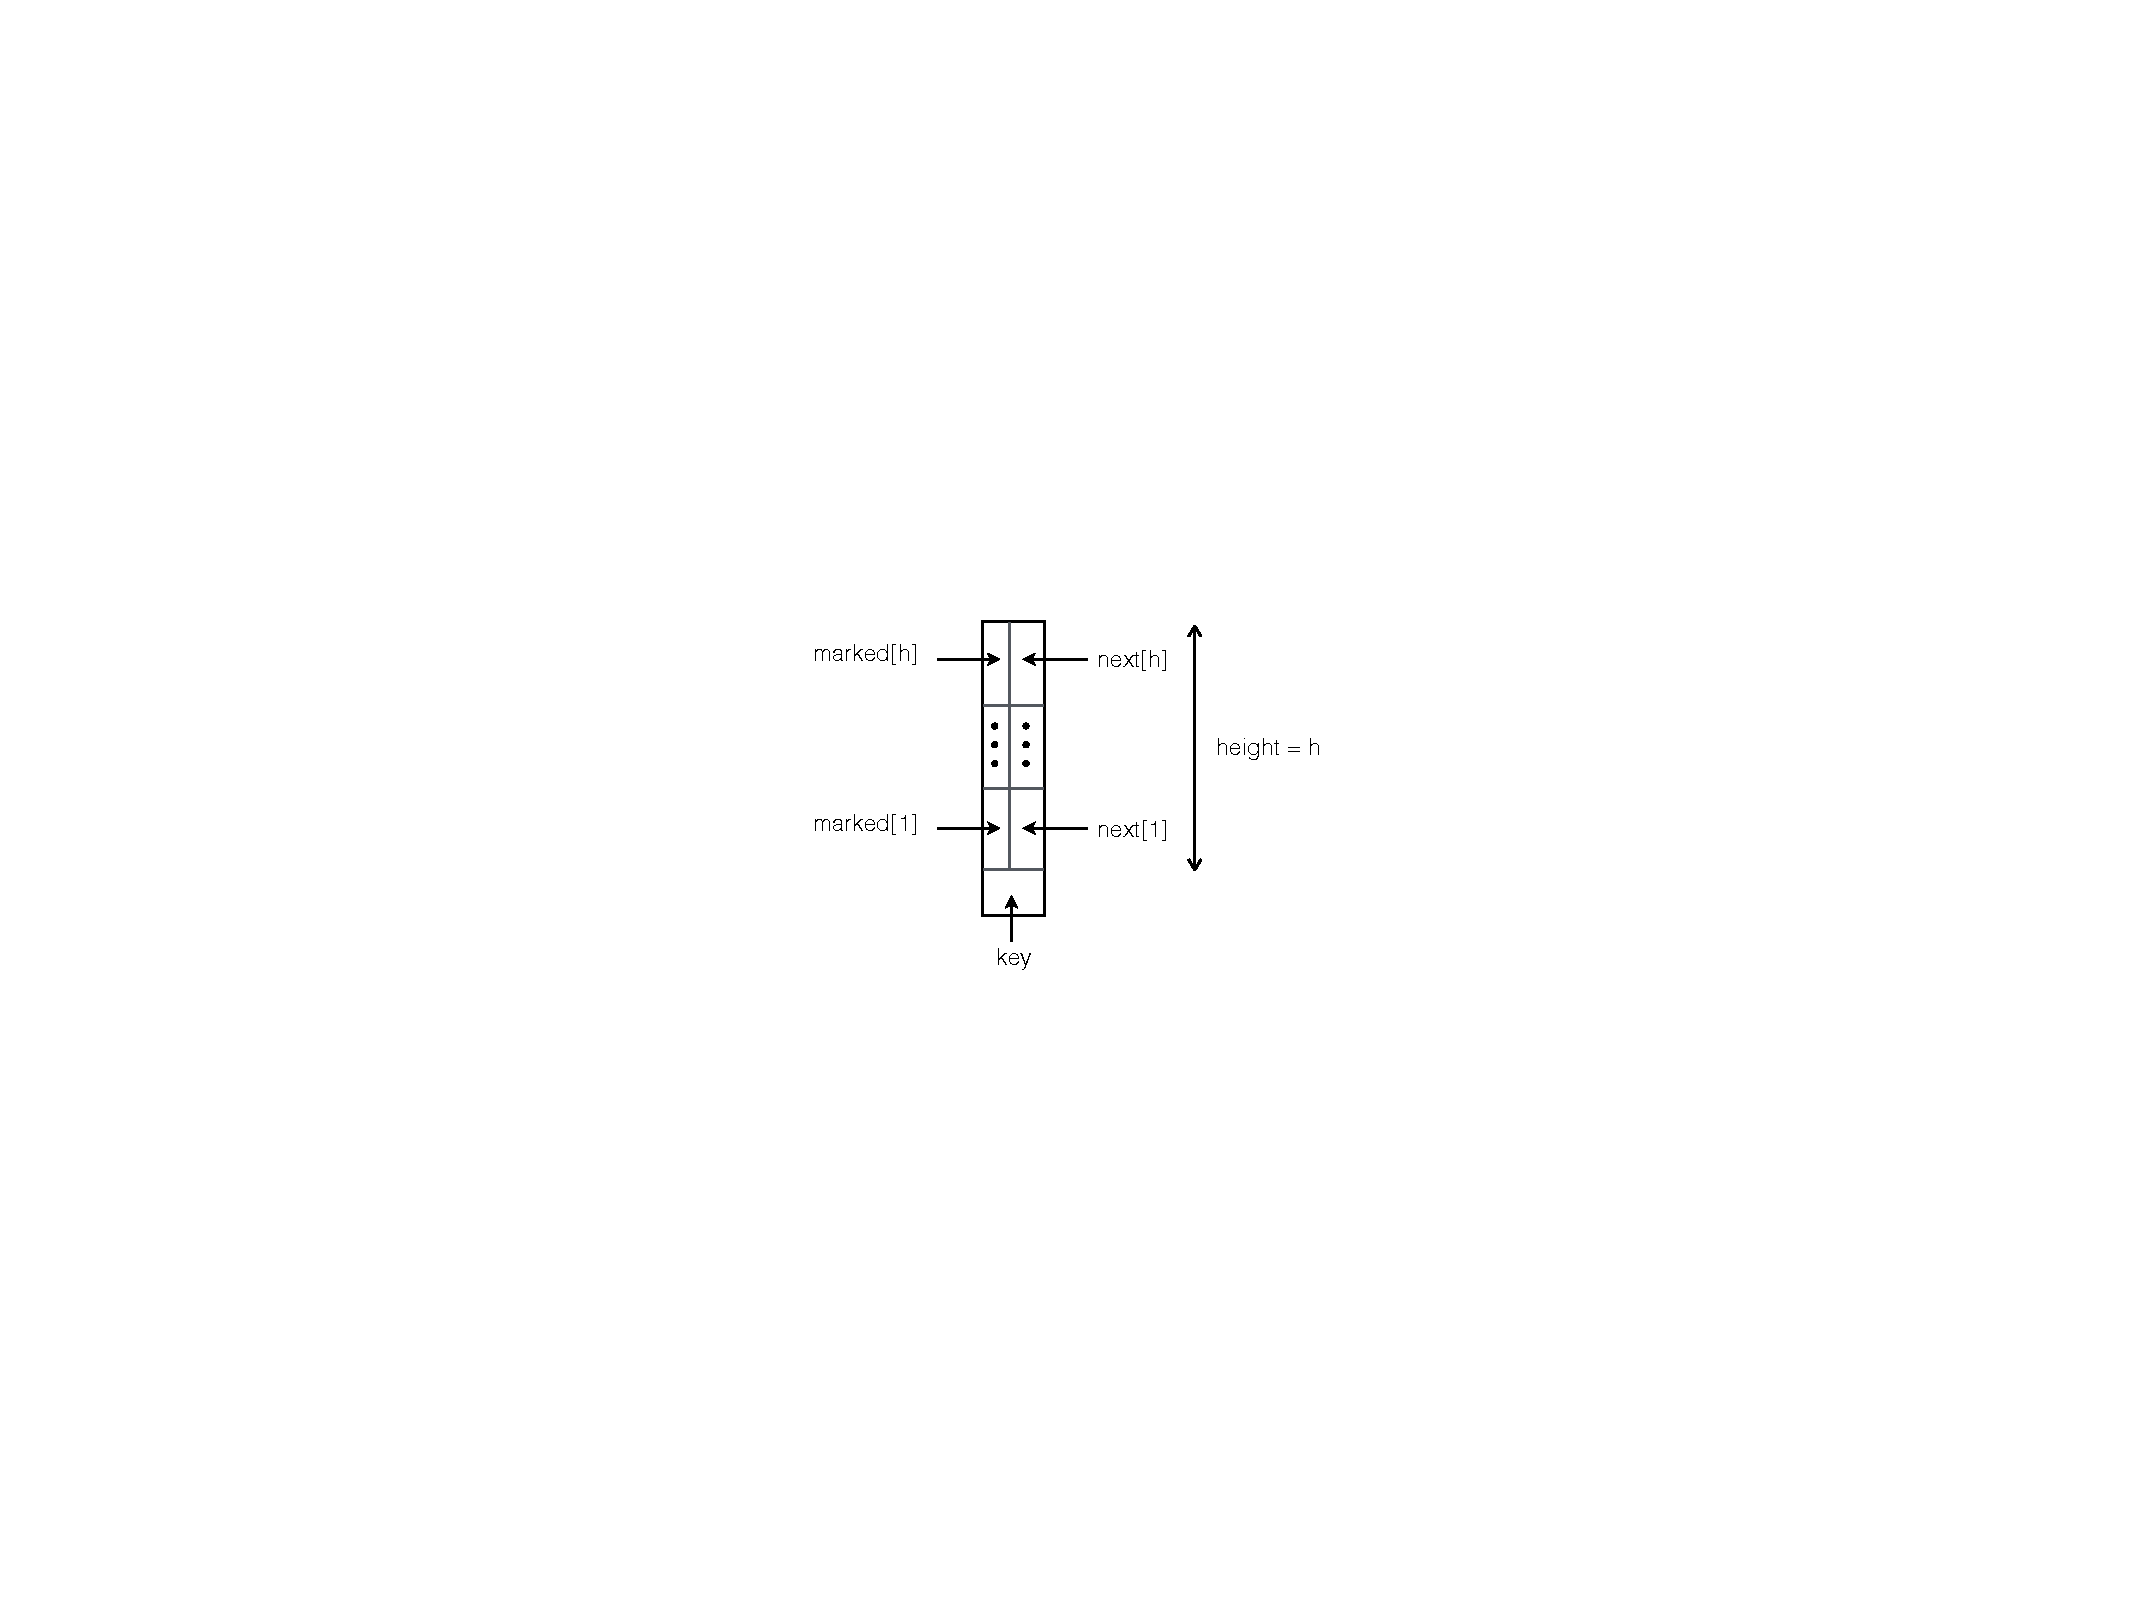
\includegraphics[width=0.4\textwidth, trim={13cm 10cm 12cm 9cm}, clip]{skipcell.pdf}  
\vspace*{-0.6cm}
    \caption{A structure of a cell}
    \label{skipcell}
  \end{center}
  \vspace{-40pt}
  \vspace{1pt}
\end{wrapfigure}
When applying fragment abstraction to skiplists, we  use two types of fragments:
{\em level 1-fragments} for
nodes connected by a $\tt next[1]$-pointer, and {\em higher level-fragments} for
nodes connected by a higher level pointer. In other words, we abstract all levels
higher than 2 by the abstract element $\tt higher$. Thus, a pointer or
non-pointer variable of form $\tt v[k]$, indexed by a level ${\tt k} \geq 2$, is
abstracted to as the variable $\tt v[higher]$.

Let us illustrate how fragment abstraction applies to the skiplist
algorithm.
\begin{figure}
\vspace*{-0.6cm}
\center  
 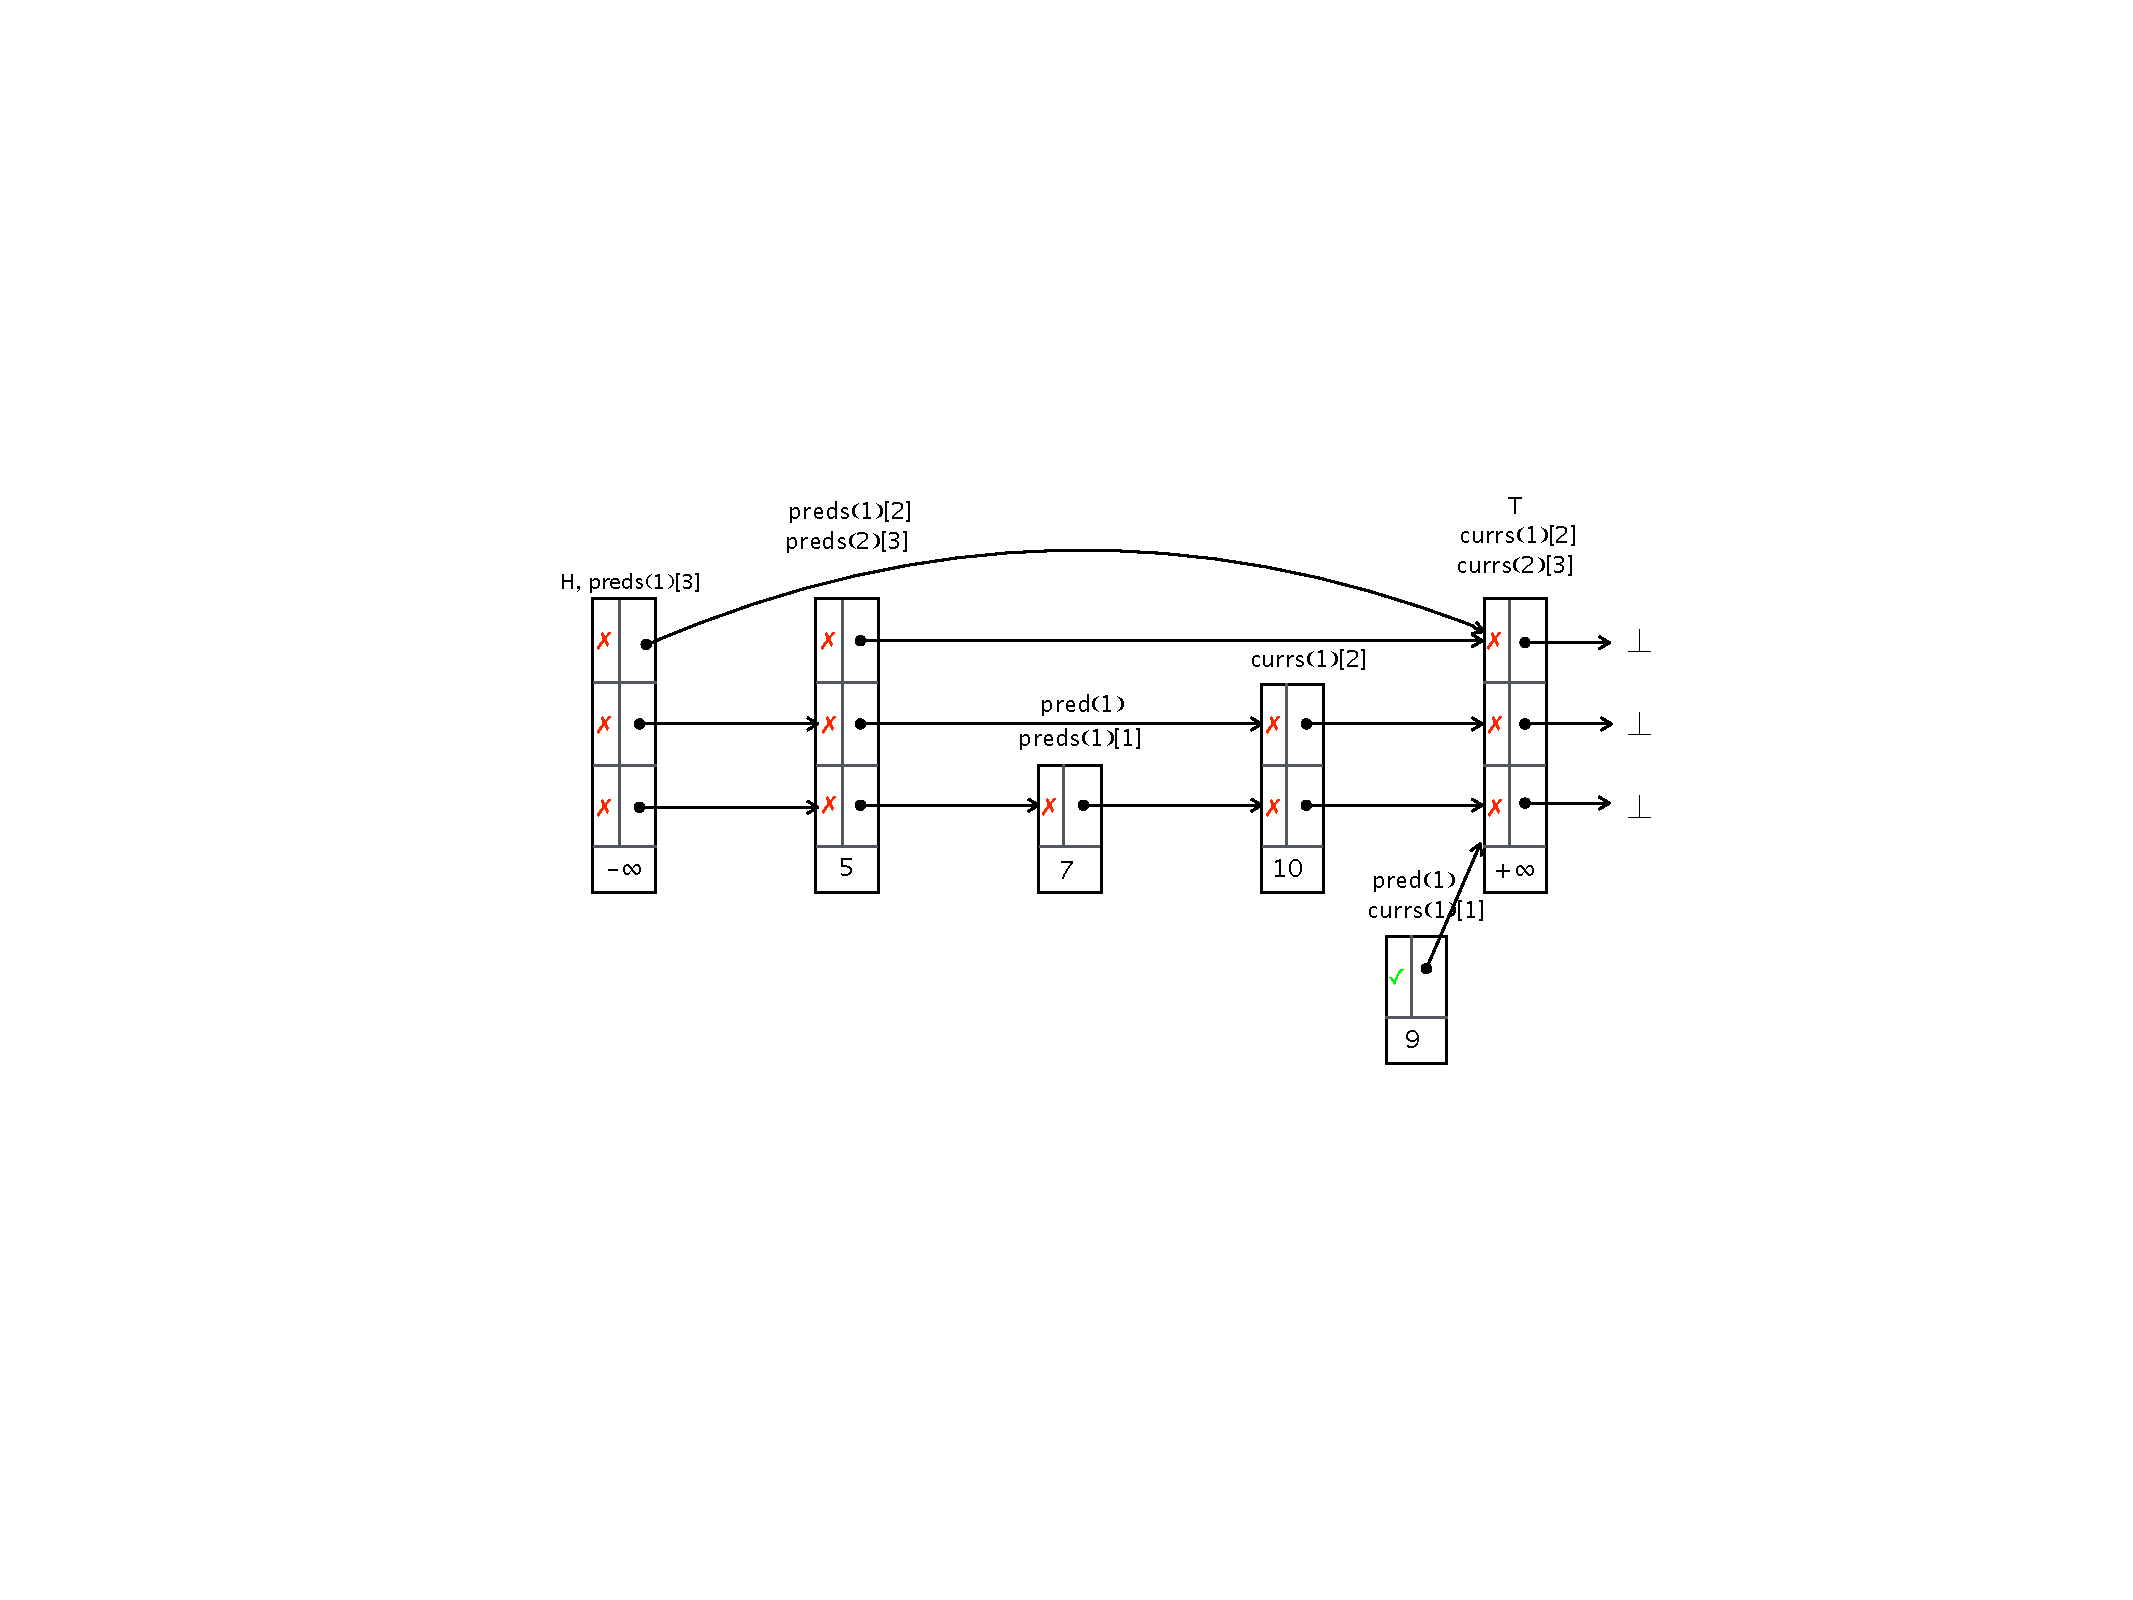
\includegraphics[width=1.2\textwidth, trim={7cm 8cm 0.5cm 6cm}, clip]{skipshape.pdf}  
\vspace*{-0.6cm}
 \caption{A concrete shape of 3-level skiplist with two threads}
\label{sl-shape}
\vspace*{-0.6cm}
\end{figure}
%\todo[inline]{Quy: you must provide example heaps, etc. before I can continue
%  writing}
Figure~\ref{sl-shape} shows an example heap state of the
skiplist algorithm with three levels. Each heap cell is shown with the values of its fields as described in Figure~\ref{skipcell}. %\bjcom{Add a legend, showing the layout of fields, as in previous papers}
In addition, each cell is labeled by the
pointer variables that point to it; we use ${\tt preds(i)[k]}$ to denote the local
variable ${\tt preds[k]}$ of thread $\thread_{\tt i}$, and the same for other local variables.
In the heap state of Figure~\ref{sl-shape}, thread $\thread_1$ is trying to add a new node of height $1$ with key $9$, and has reached line $8$ of the $\tt add$ method. Thread $\thread_2$ is trying to add a new node with key $20$ and it has done its first iteration of the loop in the $\tt find$ method in line $19$. The value of the observer register is $9$; thus it currently tracks the $\tt add$ operation of $\thread_1$.
\bjcom{Where is the node with key 20?}


%You can find some improvement of this list


%\todo[inline]{Here, explain how the fragments express these key invariants,
%maybe by picking some representative example(s)}

%The heap consists of a set of singly linked lists (SLLs), each of which
%is accessed from a pointer in the array ${\tt pools[maxThreads]}$
%in a configuration when % Quy write from here
%it is accessed concurrently by three threads $\thread_1$, $\thread_2$, and $\thread_3$. The heap consists of three SLLs accessed from the three pointers $\tt pools[1]$, $\tt pools[2]$, and $\tt pools[3]$ respectively. Each heap cell is
%shown with the values of its fields, using the layout shown to the right in
%Figure~\ref{fig:tsshape}.
%In addition, each cell is labeled by the
%pointer variables that point to it. We use ${\tt lvar[i]}$ to denote the local
%variable ${\tt lvar}$ of thread $\thread_i$.
%
%In the heap state of Figure~\ref{fig:tsshape},
%thread $\thread_1$ is trying to push a new node with data value $4$, pointed by its local variable $\tt new$, having reached line 3.
%Thread $\thread_3$ has just called the ${\tt push}$ method.
%Thread $\thread_2$ has reached line 12 in the execution of the ${\tt pop}$ method,  and has just assigned ${\tt youngest}$ to the first node in the list
%pointed to by $\tt pools[3]$ which is not logically removed (in this case it is the last node of that list).
%Not shown in Figure~\ref{fig:tsshape} is the configuration of the
%observer.
%In this case, the
%observer is the one in Figure~\ref{fig:lifostack:fig}, which has two registers
%$\tt x_1$ and $\tt x_2$, which are assigned the values $4$ and $2$,
%respectively.

%\begin{figure}
%\center  
% \input skiplistabs  
% \caption{Fragment abstraction of the skiplist algorithm}
%\label{sl-abs}
%\end{figure}


%% Let a {\em local symbolic configuration} be an abstraction of the program
%% counter and local data variables of an arbitrary thread $\thread$.
%% Our symbolic representation of a set of program configurations consists of
%% a mapping from a set of local symbolic configurations,
%% which maps each local symbolic configuration in its domain to a set of fragments.
%% A global configuration satisfies a symbolic representation $\symbrep$
%% if the view of each thread $\thread$ satisfies some local symbolic
%% configuration in the domain of $\symbrep$, which is mapped to a set
%% of fragments, which represents the heap that is accessible to $\thread$.

%% Our fragment abstraction for skiplists uses two types of fragments: {\em level 1-fragments} for
%% cells connected by a $\tt next[1]$-pointer, and {\em higher level-fragments} for
%% cells connected by a higher level pointer. This means that we abstract all levels
%% higher than 2 by the abstract element $\tt higher$.
%\todo[inline]{Fix the wrapfigure!!}
Figure~\ref{fig:skiplistabs} illustrates how pairs of heap nodes can be represented by fragments.
As a first example, in the view of thread $\thread_1$, the two left-most cells
in Figure~\ref{sl-shape} are represented by the level 1-fragment $\frag_1$ in Figure~\ref{fig:skiplistabs}.
Here, the variable $\tt preds(1)[3]$ is represented by $\tt preds[higher]$. The mapping $\pi_1$ represents the data abstraction of
the $\tt key$ field, here saying that it is smaller than the value $9$ of the
observer register.
The two left-most cells are also represented by
a higher-level fragment, viz.\ $v_8$.
The pair consisting of the two sentinel cells (with keys $\tt -\infty$ and $\tt +\infty$) is represented by the higher-level fragment $v_9$. In each fragment, the abstraction $\vals$ of non-pointer fields are shown represented inside each tag of the fragment. The $\datarelat{\frag}$ is shown as a label on the  arrow between two tags. Above each tag is $\pvars$. The first row under each tag is $\reachfrom$, whereas the second row is $\reachto$.
 

%In the fragment, we have 
%\begin{itemize}
%\item $\tt i.\vals(key): x \mapsto {<}$, $\tt o.\vals(key): x \mapsto {<}$, $\tt i.\vals(marked) =\; $\cross, $\tt o.\vals(marked) = \;$\cross
%\item  $\tt i.\pvars = \{H, preds[higher]\}$, $\tt o.\pvars = \{preds[higher]\}$,
%\item   $\tt i.\reachfrom = \{H\}$, $\tt i.\reachfrom = \{H\}$	 
%\item   $\tt i.\reachto = \{T\}$, $\tt o.\reachto = \{T\}$	
%\item  $\tt i.\private = \{false\}$, $\tt o.\private = \{false\}$
%\end{itemize} 
%The pair of heap cells with keys $\tt -\infty$ and $\tt +\infty$ in the level 3 is represented by $\frag_8$ where the variable $\tt preds(1)[3]$ is represented by $\tt preds[higher]$. In the fragment, we have
% \begin{itemize}
%\item $\tt i.\vals(key): x \mapsto {<}$, $\tt o.\vals(key): x \mapsto {<}$, $\tt i.\vals(marked) =\; $\cross, $\tt o.\vals(marked) = \;$\cross
%\item  $\tt i.\pvars = \{H, preds[higher]\}$, $\tt o.\pvars = \{T, currs[higher]\}$,
%\item   $\tt i.\reachfrom = \{H\}$, $\tt i.\reachfrom = \{H,T,x\}$	 
%\item   $\tt i.\reachto = \{T\}$, $\tt o.\reachto = \{T\}$	
%\item  $\tt i.\private = \{false\}$, $\tt o.\private = \{false\}$
%\end{itemize}
\begin{figure}
\center
	\input skiplistabs
\caption{Fragment abstraction of skiplist algorithm}
\label{fig:skiplistabs}
\vspace*{-0.6cm}
\end{figure} 
Figure~\ref{fig:skiplistabs} shows a set of fragments that is sufficient to
represent the part of the heap that is accessible to
$\thread_1$ in the configuration in Figure~\ref{sl-shape}. There are $11$ fragments, named $\frag_1$, \ldots , $\frag_{11}$. Two of
these ($\frag_6$, $\frag_7$ and $\frag_{11}$) consist of a tag that points to $\dangconst$. All other fragments consist of a pair of pointer-connected tags. The fragments $\frag_1$, \ldots , $\frag_{6}$ are  level-1-fragments, whereas $\frag_7$, \ldots , $\frag_{11}$ are higher level-fragments. The $\tt private$ field of the input tag of $\frag_7$ is $\tt true$, whereas the $\tt private$ field of tags of other fragments are $\tt false$.

To verify linearizability of the algorithm in Figure~\ref{sl-code:fig},
we must represent several key invariants of the heap. These include (among others):
\begin{enumerate}
\item the bottom-level list is strictly sorted in $\tt key$ order,
  %% Two unmarked nodes cannot have the same $\tt key$.
\item a higher-level pointer from a globally reachable node is a shortcut into the level-1 list, i.e.,
  it points to a node that is reachable by a sequence of $\tt next[1]$ pointers,
\item all nodes which are unreachable from the head of the list are marked,
  and
\item the variable $\tt pred$ points to a cell whose $\tt key$ field is never
  larger than the input parameter of its $\tt add$ method.
%% \item The variable $\tt pred$, $\tt curr$, $\tt preds$, $\tt currs$ reflect the position of the
%%   cell with $\tt key$
\end{enumerate}
Let us illustrate how such invariants are captured by our fragment abstraction.
\begin{inparaenum}[1)]
\item
  All level-1 fragments are strictly sorted, implying that the bottom-level list is strictly sorted.
\item
  For each higher-level fragment $\tt v$, if $\tt H \in \tt v.i.\reachfrom$ then also $\tt H \in \tt v.o.\reachfrom$,
  implying (together with $\tt v.\phi = \set{<}$)
  that the cell represented by $\tt v.o$ it is reachable from that represented by $\tt v.i$
  by a sequence of $\tt next[1]$-pointers.
\item
  This is verified by inspecting each tag: $\frag_{3}$ contains the only unreachable tag, and it is also marked.
\item
  The fragments express this property in the case where the value of $\tt key$ is
  the same as the value of the observer register $\tt x$. 
 Since the invariant holds for any value of $\tt x$, this property
  is sufficiently represented for purposes of verification.
%% Finally, the last invariant is expressed by the fact that $\tt x$ is larger than data fields of all tags containing $\tt pred$,$\tt preds$, and $\tt x$ is smaller than or equal to data fields of all tags containing $\tt curr$,$\tt currs$.     
\end{inparaenum}

%\todo[inline]{The below is for TS Stack. To be rmeoved and replaced}
%\begin{itemize}
%\item The $\tt data$ field of the tag (to the left) abstracts the data value
%  $2$ to the set of observer registers with that value: in this case
%  $\reg_2$.
%\item The $\tt ts$ field (at the top) abstracts the timer value $15$ to
%  the possible relations with $\tt ts$-fields of heap cells with the same
%  data value as each observer registers. Recall that observer registers
%  $\reg_1$ and $\reg_2$ have values $4$ and $2$, respectively. There are
%  three heap cells with $\tt data$ field value $4$, all with a $\tt ts$
%  value less than $15$. There is one heap cell with
%  $\tt data$ field value $2$, having $\tt ts$ value $15$.
%  Consequently, the abstraction of the $\tt ts$ field maps $\reg_1$ to
%  $\set{>}$ and $\reg_2$ to $\set{=}$: this is shown as the mapping
%  $\lambda_4$ in Figure~\ref{fig:tsviewshape}.
%\item The $\tt mark$ field assumes values from a small finite domain and
%  is represented precisely as in concrete heap cells
%\end{itemize}
%Above the top, the tag contains the thread-local and global pointer variables
%that point to the cell, in this case $\tt youngest$ and $\tt n$.
%At the bottom of the tag, the first row contains the global variables 
%pointing to cells from which the cell can be reached, in this case
%$\tt pools[3]$, as well as observer registers whose value is equal to the
%${\tt data}$ field of a cell from which  the cell can be reached, in this
%case $\reg_2$ (since the cell itself has the same data value as $\reg_2$).
%The second row contains dual information: now for cells that can be reached
%from the cell itself (this is again $\reg_2$).
%
%\todo[inline]{Fix the issue with ${\tt pools[3]}$}
%
%Each cell in the heap state of Figure~\ref{fig:tsshape} now satisfies
%some tag in Figure~\ref{fig:tsshape}. Moreoever, each pair of pointer-connected
%cells (where the pointed-to ``cell'' can also be $\dangconst$)
%satisfies some fragment in Figure~\ref{fig:tsshape} in the obvious way.
%Conversely, the set of fragments in
%Figure~\ref{fig:tsshape} represents the set of heaps in which each pair of
%pointer-connected cells satisfies one of its fragments. For instance, the
%list pointed to by $\tt pools[3]$ is represented by the sequence of
%fragments $\frag_4 \frag_5 \frag_6 \frag_7$.
%
%\todo[inline]{Maybe we should omit the rest of this section?}
%In order to obtain a complete representation of reachable program configurations,
%we must also represent the local states of a thread. This is done in a standard
%manner, by applying the same data abstraction as for heap cells. For instance,
%the local state of thread $\thread_2$ corresponding to
%Figure~\ref{fig:tsshape} is represented by a {\em local symbolic configuration}
%that contains the values of the program counter and variable $\tt success$,
%abstracts the value of ${\tt k}$ into the set $\set{{\tt me},{\tt ot}}$ and
%applies the timestamp abstraction to ${\tt maxTS}$.
%
%%% We are now ready to present our symbolic representation of a set of
%%% reachable program configurations. 
%%% %% It maps each local symbolic configuration to a set of fragments, which
%%% %% is a symbolic representation of the set of corresponding reachable heaps.
%%% Our symbolic representation is a mapping from a set of local symbolic
%%% configurations, which maps each local symbolic configuration in its domain
%%% to a set of fragments.
%%% A global configuration satisfies a symbolic representation $\symbrep$
%%% if the local state of each thread $\thread$ satisfies some local symbolic
%%% configuration in the domain of $\symbrep$, which is mapped to a set
%%% of fragments, which is satisfied by heap wrp.\ to thread $\thread$.
%
%
%%% Our symbolic representation represents the reachable local states of a thread by
%%% a finite set of {\em local symbolic configurations}, using our
%%% data abstraction.
%%% It maps each local symbolic configuration to a set of fragments, which
%%% is a symbolic representation of the set of corresponding reachable heaps.
%%% Thus, our symbolic representation is a mapping from a set of local symbolic
%%% configurations, which maps each local symbolic configuration in its domain
%%% to a set of fragments.
%%% A global configuration satisfies a symbolic representation $\symbrep$
%%% if the local stat of each thread $\thread$ satisfies some local symbolic
%%% configuration in the domain of $\symbrep$, which is mapped to a set
%%% of fragments, which represents the heap that is accessible to $\thread$ in
%%% the global configuration. In the following, we explain more precisely the
%%% local symbolic configurations, and our fragment abstraction.
%
%In the  verification, we must compute a symbolic representation
%that is satisfied by all reachable program configurations (recall that
%program configurations include the state of the observer).
%This invariant is obtained by an abstract-interpretation-based
%fixpoint procedure, which starts
%from a representation of the set of initial configurations, and
%thereafter repeatedly performs
%postcondition computations that extend the
%symbolic representation by the effect of any execution step of the program,
%until convergence.
%This procedure is presented in Section~\ref{subsect:postcond}.
%
%



